\section{Epidemien in heterogenen Populationen}
\label{sec:epidemiology-heterogen}

\begin{code}
	\caption{Skript für die Simulation des SIR-Modells mit heterogenen Populationen.}
	\mSourceFile{\srcDir/epidemiologySIRGroupsProg.m}
	\label{source:epidemiology-sir-groups-program}
\end{code}

\begin{code}
	\caption{Funktion zur Berechnung des SIR-Modell mit heterogenen Populationen}
	\mSourceFile{\srcDir/epidemiologySIRGroups.m}
	\label{source:epidemiology-sir-groups}
\end{code}
\ \newpage


\begin{figure}[h]
	\centering
	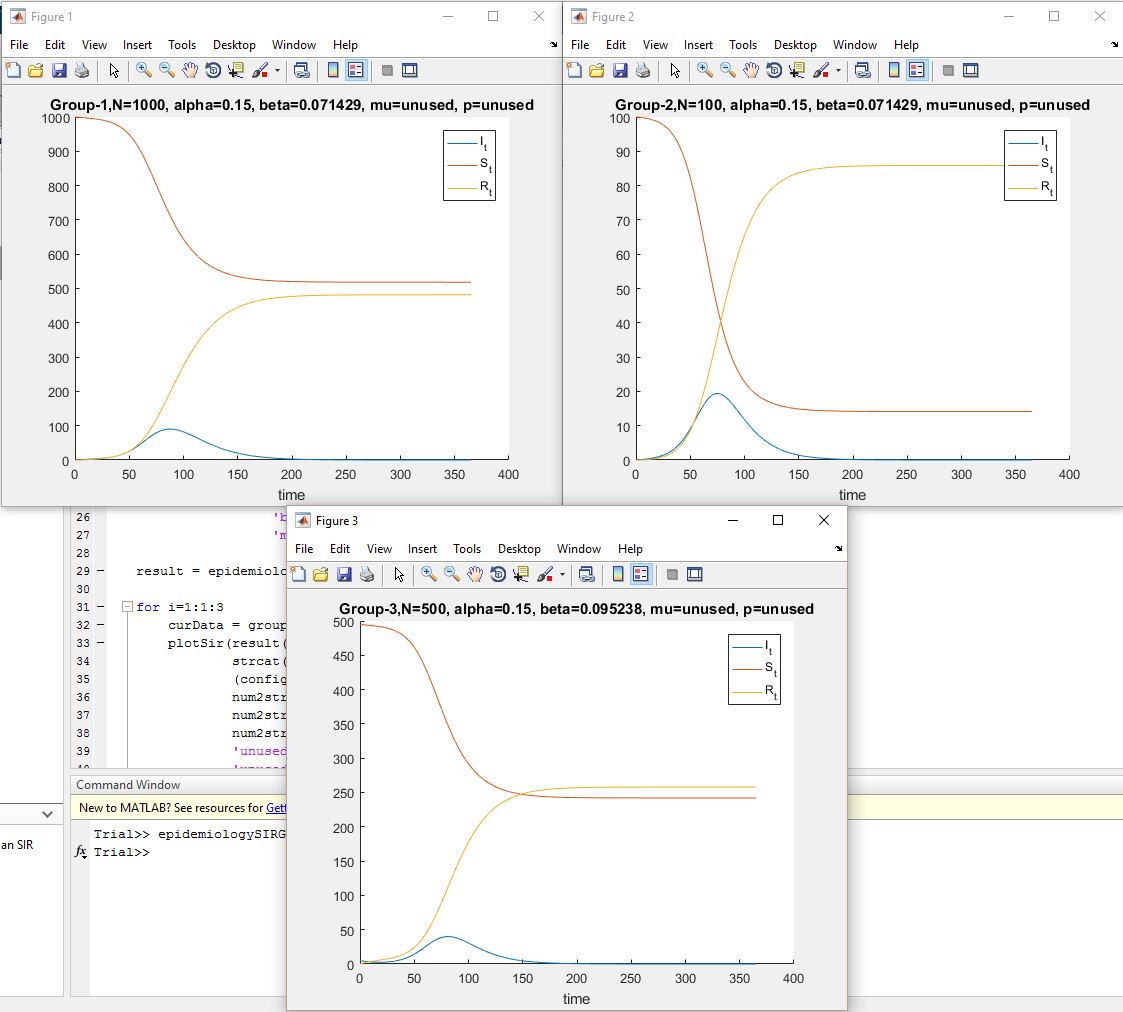
\includegraphics[scale=0.55]{\imageDir/epiomology-sir-groups.JPG}
	\caption{Verlauf der Epidemie in den verschiedenen Gruppen mit einem SIR-Modell}
	\label{test:epidemiology-sir}
\end{figure}

